\setcounter{section}{41}

\section{Применение формулы обращения Мёбиуса для подсчета числа циклических последовательностей.}

Пусть $V$ - множество всех линейных последовательностей (не циклических) длины n. $d_1, \dots, d_s$ - делители числа n, тогда $V = V_1 \cup \dots \cup V_s$, где $V_i$ - множество линейных последовательностей с периодом $d_i$. Положим $W_i$ - множество всех линейных последовательностей длины $d_i$ и периода $d_i$. Очевидно, что $|V_i| = |W_i|$. Пусть $U_i$ - множество циклических последовательностей, которые получаются из последовательностей $W_i$ циклическим сдвигом. Тогда $d_i|U_i| = |W_i|$. Пусть есть функция $M(d_i) = |U_i|$ - число циклич. последовательностей, которые получаются из обычных последовательностей длины d, периода d. Рассмотрим функцию \[r^n =  \sum_{i=1}^s |W_i| = \sum_{i=1}^s d_i|U_i| = d_1M(d_1) + \dots + d_sM(d_s) = \sum_{d|n} dM(d)\]
Тогда возьмём $g(n) = r^n$, $f(n) = nM(n)$. Получается, что $g(n) = \sum_{d|n}f(d)$ . Применима ф-ла обращ. Мёбиуса: \[f(n) = nM(n) = \sum_{d|n} \mu (d)g(\frac{n}{d}) =   \sum_{d|n} \mu (d) r^{n/d} \Rightarrow  M(n) = \frac{1}{n} \sum_{d|n} \mu (d) r^{n/d}\]
M(n) - циклические последовательности, отвечающие словам длины n и периода n. Пусть $T_r(n)$ - искомая величина, количество всех циклических слов над алфавитом из r букв, имеющих длину n: \\
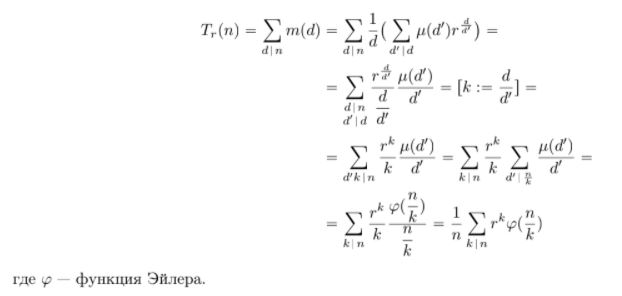
\includegraphics{images/42}

\section{Функция Мёбиуса на ч.у.м. Совпадение функции Мёбиуса $\mu(1, n)$ на ч.у.м. $\langle$N, $\vdots$ $\rangle$ и обычной функции Мёбиуса $\mu(n)$ на $ \mathbb{N}$ (для всех n). Общая формула обращения Мёбиуса для частично упорядоченных множеств (б/д).}

$(P, \preceq)$ - ч.у.м., причём $\forall p \in P$  $\exists$ лишь конечное число $p' \in P: p' \preceq p$. Тогда \textbf{ф-ия Мёбиуса на ч.у.м.}: \[x, y \in P: x \preceq y, \mu(x, y) = \left\{
  \begin{array}{ccc}
    1, x = y \\
    - \sum_{x \preceq z \prec y} \mu(x, z), x \neq y\\
  \end{array}
\right. \] \par
"Классическая"  функция Мёбиуса $\overline{\mu}(x)$ на $ \mathbb{N}$:
\[ 
\overline{\mu}(x)= \left\{
  \begin{array}{ccc}
    1, x = 1 \\
    (-1)^s, x = p_1\dots p_ s\\
    0 \\
  \end{array}
\right.
\] \par
Докажем, что на ч.у.м. $\langle$N, $\vdots$ $\rangle$ $\mu (x, y) = \overline{\mu}(y/x)$. \par
$\blacktriangle$
Доказательство мат. индукцией по величине дроби $y/x$
$\mu (x, y) = 1 = \overline{\mu}(x/x) = \overline{\mu}(1)$;
Теперь $x \prec y$, т.е. $x|y$, но $x \neq y \Rightarrow y = x*p_1^{a_1}*\dots*p_s^{a_s}$ согласно основной теореме арифметики. Тогда 
$ \mu(x, y) = - \sum_{x \preceq z \prec y} \mu(x, z) $, причём $z = x*p_1^{\beta_1}*\dots*p_s^{\beta_s}$, $0 \leqslant \beta_i \leqslant a_i$, $z/x < y/x$. Тогда по предположению индукции 
\[ \mu(x, y) = - \sum_{x \preceq z \prec y} \mu(x, z) = - \sum_{x \preceq z \prec y} \overline{\mu}(z/x) = - \sum_{x \preceq z \prec y} \overline{\mu}(p_1^{\beta_1}*\dots*p_s^{\beta_s}) = \left\{
  \begin{array}{ccc}
   -\sum_{i=0}^{s-1} (-1)^iC_s^i = (-1)^{s+2} = (-1)^s, a_1=\dots=1 \\
   -\sum_{i=0}^{s} (-1)^iC_s^i = 0\\
  \end{array}
\right.\]
$\blacksquare$ \par
\textbf{Обобщённая формула обращения Мёбиуса для ч.у.м.}: Пусть $g(y) = \sum_{x\preceq y} f(x)$. Тогда $f(y) = \sum_{x\preceq y} \mu(x, y)g(x)$

\section{Формула Мёбиуса на ч.у.м. Вывод формулы $\sum_{a\preceq z \preceq b} \mu(z, b) = \left\{
  \begin{array}{ccc}
   1, a=b \\
   0, a<b \\
  \end{array}
\right.$}

$\blacktriangle$
1. $a \prec b$ - между a и b нет элементов ч.у.м. Тогда $\sum_{a\preceq z \preceq b} \mu(z, b) = \mu(a, b) + \mu(b, b) = -\sum_{a \preceq u \prec b} \mu(a, u) + 1 = -\mu(a, a) +1 = -1 + 1 = 0 $ - база индукции.
Индукция по длине максимальной цепи между данными элементами ч.у.м. a и b.
\[ \sum_{a\preceq z \preceq b} \mu(z, b) = \mu(b, b) + \sum_{a\preceq z \prec b} \mu(z, b) = 1 - \sum_{a\preceq z \prec b} \sum_{z\preceq u \prec b} \mu(z, u) = 1 - \sum_{a\preceq u \prec b} \sum_{a\preceq z \prec u} \mu(z, u) = 1 - 1 - \sum_{a\prec u \prec b} \sum_{a\preceq z \prec u} \mu(z, u) = 0\]
$\blacksquare$

\section{Формула Мёбиуса на ч.у.м. Обобщёная формула обращения Мёбиуса}
Доказательство формулы Мёбиуса на ч.у.м.: \\ \par
$\blacktriangle$
$\sum_{x \preceq y} \mu(x, y)(\sum_{z \preceq x} f(z)) = \sum_{(z, x): z \preceq x \preceq y} \mu(x, y)f(z) = \sum_{z \preceq y}f(z) * (\sum_{z \preceq x \preceq y} \mu(x, y)) = f(y)*1 + \sum_{z \prec y}f(z) * (\sum_{z \preceq x \preceq y} \mu(x, y)) = f(y) + 0 = f(y)$
$\blacksquare$

\section{Передоказательство формулы включений и исключений при помощи формулы обращения Мёбиуса на ч.у.м. Определение множества X, порядка $\preceq$. Вычисление функции Мёбиуса на данном ч.у.м.}

Рассмотрим ч.у.м.: $(2^{\{1, \dots, n\}}, \subseteq)$. Вычислим функцию Мёбиуса. Рассмотрим множества $A_1, \dots, A_n, A = A_1 \cup \dots \cup A_n$; $P = \{1, \dots, n \}$. \par
Разберёмся с формулой Мёбиуса на данном ч.у.м. Рассмотрим $I' \subseteq I \subseteq \{1, \dots, n\}$. Тогда $\mu(I', I) = (-1)^{|I|-|I'|}$ \par
$\blacktriangle$
Докажем индукцией по $|I| - |I'|$. База: I = I' (очевидна). \\
$|I| - |I'| = k > 0$. Тогда $\mu(I', I) = -\sum_{I' \preceq I'' \prec I}\mu(I', I'')$. $|I''| - |I'| < k \Rightarrow$ по предположению индукции $\mu(I', I'') = (-1)^{|I''| - |I'|}$. Очевидно, что $|I''| \geqslant |I'|$. Тогда возникает вопрос, если мы зафиксируем $l = |I''|, l = |I'|, |I'| + 1, \dots, |I'| + k - 1$, сколькими способами можно будет выбрать $I''$ при фиксированном $I'$? Очевидно, $C_k^{l - |I'|} = C_k^m$, где $m = l - |I'| = 0, \dots, k - 1$. Тогда 
\[ \mu(I', I) = -\sum_{I' \preceq I'' \prec I}\mu(I', I'') = -\sum_{m=0}^{k-1}(-1)^m C_k^m = -(-1)^{k+1} = (-1)^k\]
$\blacksquare$

\section{Передоказательство формулы включений и исключений при помощи формулы обращения Мёбиуса на ч.у.м. Формула для вычисления функции Мёбиуса на данном ч.у.м.(б/д). Вывод формулы включений и исключений.}

$f(I \subset P) :=$ количество элементов из A, которые могут не принадлежать $A_i, i \in I$, но обязательно принадлежат всем остальным. Так, $f(P) = |A|$; если же $I \neq P$: $f(I) = |\bigcap_{i \notin I} A_i|$ \par
$g(I \subset P) :=$ количество элементов из А, которые обязаны не принадлежать $A_i, i \in I$, и обязаны принадлежать всем остальным. $f(I) = \sum_{I' \subseteq I} g(I')$; $g(\{1, \dots, n\}) = 0$\par 
Формула обращения Мёбиуса: $f(y) = \sum_{x\preceq y}g(x) \Rightarrow g(y) = \sum_{x \preceq y} \mu(x, y)f(x)$. Применим её:
$ f(I) = \sum_{I' \subseteq I}g(I') \Rightarrow g(I) = \sum_{I' \subseteq I} \mu(I', I)f(I')$.
Рассмотрим $I = \{1, \dots, n\}$. $0 = \sum_{I' \subseteq \{1, \dots, n\}}f(I') = |A| + \sum_{I' \subset \{1, \dots, n\}}\mu(I', \{1, \dots, n\})|\bigcap_{i \notin I'} A_i|$. \par
Это значит, что 
\[ |A| = - \sum_{I' \subset \{1, \dots, n\}}\mu(I', \{1, \dots, n\})|\bigcap_{i \notin I'} A_i| = - \sum_{I' \subset \{1, \dots, n\}} (-1)^{n-|I'|} |\bigcap_{i \notin I'} A_i| =\] \[= \sum_{I' \subset \{1, \dots, n\}} (-1)^{n-|I'| + 1} |\bigcap_{i \notin I'} A_i| = \sum_{I'' \neq \varnothing} (-1)^{|I''|+1} |\bigcap_{i \in I''} A_i|, I'' = \{1, \dots, n\} \setminus I'\]